\begin{figure}[ht!]
    \begin{center}
        % This file was created by matlab2tikz.
%
%The latest updates can be retrieved from
%  http://www.mathworks.com/matlabcentral/fileexchange/22022-matlab2tikz-matlab2tikz
%where you can also make suggestions and rate matlab2tikz.
%
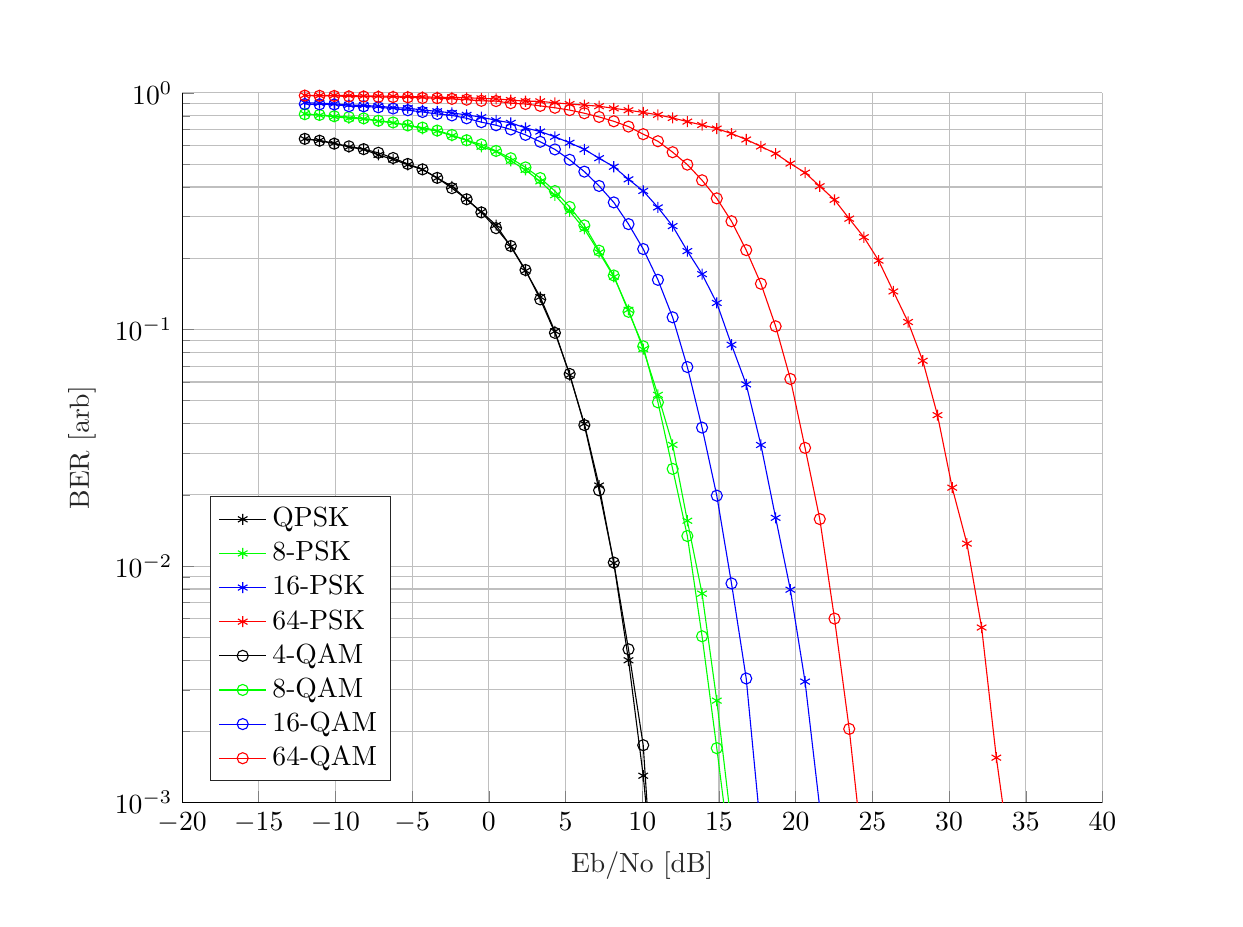
\begin{tikzpicture}

\begin{axis}[%
width=4.602in,
height=3.549in,
at={(0.772in,0.479in)},
scale only axis,
xmin=-20,
xmax=40,
xlabel style={font=\color{white!15!black}},
xlabel={Eb/No [dB]},
ymode=log,
ymin=0.001,
ymax=1,
yminorticks=true,
ylabel style={font=\color{white!15!black}},
ylabel={BER [arb]},
axis background/.style={fill=white},
axis x line*=bottom,
axis y line*=left,
xmajorgrids,
ymajorgrids,
yminorgrids,
legend style={at={(0.03,0.03)}, anchor=south west, legend cell align=left, align=left, draw=white!15!black}
]
\addplot [color=black, mark=asterisk, mark options={solid, black}]
  table[row sep=crcr]{%
-12	0.63916804159792\\
-11.0408163265306	0.629618519074047\\
-10.0816326530612	0.612669366531675\\
-9.12244897959184	0.5907204639768\\
-8.16326530612245	0.576921153942304\\
-7.20408163265306	0.546522673866306\\
-6.24489795918367	0.523523823808809\\
-5.28571428571429	0.496975151242438\\
-4.3265306122449	0.474226288685566\\
-3.36734693877551	0.43642817859107\\
-2.40816326530612	0.402829858507074\\
-1.44897959183673	0.355032248387581\\
-0.489795918367347	0.314334283285836\\
0.469387755102041	0.276136193190341\\
1.42857142857143	0.223988800559972\\
2.38775510204082	0.177091145442728\\
3.3469387755102	0.137093145342733\\
4.30612244897959	0.0981950902454876\\
5.26530612244898	0.064146792660367\\
6.22448979591837	0.03994800259987\\
7.18367346938776	0.0218989050547473\\
8.14285714285714	0.0102994850257487\\
9.10204081632653	0.00399980000999949\\
10.0612244897959	0.00129993500324984\\
10.6846747106505	0.000501187233627271\\
};
\addlegendentry{QPSK}

\addplot [color=green, mark=asterisk, mark options={solid, green}]
  table[row sep=crcr]{%
-12	0.816109194540275\\
-11.0408163265306	0.8041597920104\\
-10.0816326530612	0.793210339483027\\
-9.12244897959184	0.781060946952653\\
-8.16326530612245	0.776511174441277\\
-7.20408163265306	0.760011999400029\\
-6.24489795918367	0.746962651867406\\
-5.28571428571429	0.731113444327782\\
-4.3265306122449	0.705164741762912\\
-3.36734693877551	0.68981550922454\\
-2.40816326530612	0.658917054147293\\
-1.44897959183673	0.630818459077046\\
-0.489795918367347	0.591720413979302\\
0.469387755102041	0.565271736413179\\
1.42857142857143	0.51622418879056\\
2.38775510204082	0.472326383680816\\
3.3469387755102	0.422628868556572\\
4.30612244897959	0.369281535923204\\
5.26530612244898	0.316134193290336\\
6.22448979591837	0.265986700664966\\
7.18367346938776	0.211889405529723\\
8.14285714285714	0.167041647917604\\
9.10204081632653	0.121093945302735\\
10.0612244897959	0.0825458727063646\\
11.0204081632653	0.0529473526323684\\
11.9795918367347	0.0325483725813709\\
12.9387755102041	0.015549222538873\\
13.8979591836735	0.00764961751912404\\
14.8571428571429	0.00269986500674966\\
15.8163265306122	0.000799960001999899\\
};
\addlegendentry{8-PSK}

\addplot [color=blue, mark=asterisk, mark options={solid, blue}]
  table[row sep=crcr]{%
-12	0.909604519774011\\
-11.0408163265306	0.904604769761515\\
-10.0816326530612	0.899005049747515\\
-9.12244897959184	0.889205539723017\\
-8.16326530612245	0.884155792210388\\
-7.20408163265306	0.879306034698265\\
-6.24489795918367	0.866156692165393\\
-5.28571428571428	0.861756912154395\\
-4.3265306122449	0.846257687115644\\
-3.36734693877551	0.835808209589523\\
-2.40816326530612	0.82245887705615\\
-1.44897959183674	0.807409629518523\\
-0.489795918367349	0.789560521973898\\
0.469387755102041	0.765711714414278\\
1.42857142857143	0.746912654367279\\
2.38775510204082	0.71126443677816\\
3.3469387755102	0.686365681715912\\
4.30612244897959	0.652167391630418\\
5.26530612244898	0.6155192240388\\
6.22448979591837	0.57717114144293\\
7.18367346938776	0.529573521323933\\
8.14285714285714	0.487325633718315\\
9.10204081632653	0.431178441077948\\
10.0612244897959	0.385080745962702\\
11.0204081632653	0.327983600819958\\
11.9795918367347	0.27353632318384\\
12.9387755102041	0.214439278036098\\
13.8979591836735	0.171391430428479\\
14.8571428571429	0.129443527823609\\
15.8163265306122	0.0861956902154891\\
16.7755102040816	0.0585970701464926\\
17.734693877551	0.032498375081246\\
18.6938775510204	0.015999200039998\\
19.6530612244898	0.00794960251987401\\
20.6122448979592	0.0032498375081246\\
21.5714285714286	0.000949952502374883\\
};
\addlegendentry{16-PSK}

\addplot [color=red, mark=asterisk, mark options={solid, red}]
  table[row sep=crcr]{%
-12	0.976551172441383\\
-11.0408163265306	0.97385130743463\\
-10.0816326530612	0.975251237438123\\
-9.12244897959184	0.973651317434127\\
-8.16326530612245	0.97070146492675\\
-7.20408163265306	0.970401479926008\\
-6.24489795918367	0.967451627418637\\
-5.28571428571428	0.966551672416381\\
-4.3265306122449	0.962551872406376\\
-3.36734693877551	0.958202089895503\\
-2.40816326530612	0.957502124893755\\
-1.44897959183673	0.95330233488326\\
-0.489795918367349	0.947952602369877\\
0.469387755102041	0.942802859857005\\
1.42857142857143	0.932653367331636\\
2.38775510204082	0.922003899805008\\
3.3469387755102	0.921003949802509\\
4.30612244897959	0.907904604769767\\
5.26530612244898	0.897105144742768\\
6.22448979591837	0.887505624718767\\
7.18367346938776	0.87850607469627\\
8.14285714285715	0.860056997150139\\
9.10204081632654	0.844807759612014\\
10.0612244897959	0.826658667066653\\
11.0204081632653	0.807659617019147\\
11.9795918367347	0.783560821958904\\
12.9387755102041	0.756262186890661\\
13.8979591836735	0.731663416829157\\
14.8571428571429	0.706564671766417\\
15.8163265306122	0.673166341682916\\
16.7755102040816	0.635218239088048\\
17.734693877551	0.593720313984297\\
18.6938775510204	0.554022298885057\\
19.6530612244898	0.50277486125694\\
20.6122448979592	0.459927003649818\\
21.5714285714286	0.403179841007951\\
22.530612244898	0.35323233838308\\
23.4897959183673	0.293935303234837\\
24.4489795918367	0.245437728113594\\
25.4081632653061	0.195490225488727\\
26.3673469387755	0.144792760361981\\
27.3265306122449	0.107544622768862\\
28.2857142857143	0.0737463126843654\\
29.2448979591837	0.0434478276086197\\
30.2040816326531	0.0214489275536224\\
31.1632653061224	0.0124493775311235\\
32.1224489795918	0.00549972501374928\\
33.0816326530612	0.0015499225038748\\
34.0408163265306	0.000549972501374928\\
};
\addlegendentry{64-PSK}

\addplot [color=black, mark=o, mark options={solid, black}]
  table[row sep=crcr]{%
-12	0.639218039098046\\
-11.0408163265306	0.627968601569922\\
-10.0816326530612	0.610069496525175\\
-9.12244897959184	0.5943202839858\\
-8.16326530612245	0.578271086445677\\
-7.20408163265306	0.558222088895556\\
-6.24489795918367	0.530623468826558\\
-5.28571428571429	0.500824958752063\\
-4.3265306122449	0.475026248687565\\
-3.36734693877551	0.437378131093446\\
-2.40816326530612	0.395730213489325\\
-1.44897959183673	0.35513224338783\\
-0.489795918367347	0.312534373281336\\
0.469387755102041	0.268036598170092\\
1.42857142857143	0.225338733063347\\
2.38775510204082	0.178441077946103\\
3.3469387755102	0.134093295335233\\
4.30612244897959	0.0967951602419879\\
5.26530612244898	0.0648967551622419\\
6.22448979591837	0.0394480275986201\\
7.18367346938776	0.0208989550522474\\
8.14285714285714	0.0103494825258737\\
9.10204081632653	0.00444977751112444\\
10.0612244897959	0.00174991250437478\\
10.6141416339895	0.000501187233627271\\
};
\addlegendentry{4-QAM}

\addplot [color=green, mark=o, mark options={solid, green}]
  table[row sep=crcr]{%
-12	0.812509374531272\\
-11.0408163265306	0.807109644517775\\
-10.0816326530612	0.796760161991899\\
-9.12244897959184	0.7903604819759\\
-8.16326530612245	0.780310984450778\\
-7.20408163265306	0.762411879406029\\
-6.24489795918367	0.75001249937503\\
-5.28571428571429	0.728363581820909\\
-4.3265306122449	0.713314334283285\\
-3.36734693877551	0.69301534923254\\
-2.40816326530612	0.664066796660167\\
-1.44897959183673	0.630768461576922\\
-0.489795918367347	0.605569721513925\\
0.469387755102041	0.56837158142093\\
1.42857142857143	0.529373531323433\\
2.38775510204082	0.48427578621069\\
3.3469387755102	0.43652817359132\\
4.30612244897959	0.384730763461827\\
5.26530612244898	0.329583520823959\\
6.22448979591837	0.27533623318834\\
7.18367346938776	0.215389230538473\\
8.14285714285714	0.169141542922853\\
9.10204081632653	0.118794060296985\\
10.0612244897959	0.0848957552122393\\
11.0204081632653	0.0491975401229938\\
11.9795918367347	0.0257487125643718\\
12.9387755102041	0.0133993300334983\\
13.8979591836735	0.00504974751262436\\
14.8571428571429	0.00169991500424978\\
15.8163265306122	0.000549972501374931\\
};
\addlegendentry{8-QAM}

\addplot [color=blue, mark=o, mark options={solid, blue}]
  table[row sep=crcr]{%
-12	0.896705164741766\\
-11.0408163265306	0.894305284735761\\
-10.0816326530612	0.893255337233142\\
-9.12244897959184	0.877906104694764\\
-8.16326530612245	0.877156142192887\\
-7.20408163265306	0.86905654717264\\
-6.24489795918367	0.858857057147145\\
-5.28571428571428	0.844807759612021\\
-4.3265306122449	0.830458477076147\\
-3.36734693877551	0.814309284535773\\
-2.40816326530612	0.803059847007653\\
-1.44897959183674	0.780910954452277\\
-0.489795918367349	0.752112394380284\\
0.469387755102041	0.729913504324784\\
1.42857142857143	0.700514974251286\\
2.38775510204082	0.66481675916204\\
3.3469387755102	0.621368931553423\\
4.30612244897959	0.576771161441926\\
5.26530612244898	0.521573921303937\\
6.22448979591837	0.464626768661567\\
7.18367346938776	0.404229788510576\\
8.14285714285714	0.344482775861207\\
9.10204081632653	0.278886055697214\\
10.0612244897959	0.218789060546972\\
11.0204081632653	0.162141892905354\\
11.9795918367347	0.112594370281486\\
12.9387755102041	0.0693965301734914\\
13.8979591836735	0.0384980750962453\\
14.8571428571429	0.0198490075496224\\
15.8163265306122	0.00844957752112397\\
16.7755102040816	0.00334983250837459\\
17.734693877551	0.000749962501874908\\
};
\addlegendentry{16-QAM}

\addplot [color=red, mark=o, mark options={solid, red}]
  table[row sep=crcr]{%
-12	0.973751312434379\\
-11.0408163265306	0.972251387430626\\
-10.0816326530612	0.970401479926\\
-9.12244897959184	0.966051697415129\\
-8.16326530612245	0.965351732413377\\
-7.20408163265306	0.961851907404626\\
-6.24489795918367	0.960101994900256\\
-5.28571428571428	0.957452127393631\\
-4.3265306122449	0.951752412379384\\
-3.36734693877551	0.949652517374132\\
-2.40816326530612	0.943452827358631\\
-1.44897959183674	0.935853207339633\\
-0.489795918367349	0.925653717314137\\
0.469387755102041	0.923203839808009\\
1.42857142857143	0.904654767261639\\
2.38775510204082	0.897305134743265\\
3.3469387755102	0.881155942202887\\
4.30612244897959	0.865206739663018\\
5.26530612244898	0.845657717114145\\
6.22448979591837	0.820308984550775\\
7.18367346938776	0.791210439478025\\
8.14285714285714	0.758412079396032\\
9.10204081632653	0.720413979301032\\
10.0612244897959	0.669216539173044\\
11.0204081632653	0.624668766561673\\
11.9795918367347	0.561371931403431\\
12.9387755102041	0.497475126243688\\
13.8979591836735	0.427178641067947\\
14.8571428571429	0.35823208839558\\
15.8163265306122	0.286685665716715\\
16.7755102040816	0.216489175541223\\
17.734693877551	0.156092195390231\\
18.6938775510204	0.103144842757862\\
19.6530612244898	0.061796910154492\\
20.6122448979592	0.0315984200789962\\
21.5714285714286	0.0157992100394981\\
22.530612244898	0.00599970001499927\\
23.4897959183673	0.00204989750512474\\
24.4489795918367	0.000549972501374933\\
};
\addlegendentry{64-QAM}

\end{axis}

\begin{axis}[%
width=5.938in,
height=4.354in,
at={(0in,0in)},
scale only axis,
xmin=0,
xmax=1,
ymin=0,
ymax=1,
axis line style={draw=none},
ticks=none,
axis x line*=bottom,
axis y line*=left
]
\end{axis}
\end{tikzpicture}%
        \caption{Comparison of BER for QPSK, 8PSK, 16PSK, 64PSK, 4QAM, 8QAM, 16QAM and 64QAM}
    \end{center}\label{fig:2}
\end{figure}

Figure~\ref{fig:2} shows BER for QPSK, 8PSK, 16PSK, 64PSK, 4QAM, 8QAM, 16QAM and 64QAM. The results are obtained using the Matlab script as shown in \ref{matlabs:task2}. The Graph shows as the signal strength increases the bitrate error decreases. QPSK or 4PSK is identical to 4QAM. This is because the constellation is identical. This is reflected in the results. For, configurations, (m>4), the lattice constellation of QAM provides better performance than the unit circle constellation of PSK. The higher the value of m, the greater the difference. As the number of symbols increases, the signal strength must be higher to achieve the same BER. This is due to the distance between symbols being smaller and therefore less resistant to white noise.

The outlier of this graph is 8-QAM. This is because the constellation is not square. This means that the distance between symbols varies. Due to the nature of adding probabilities, the variance in distance between symbols hence, BER, means the overall BER is slightly higher than expected. This is reflected in the graph where the BER for 8-QAM is almost the same as 8-PSK, where perhaps a larger gap might be expected.